%%%%%%%%%%%%%%%%%%%%%%%%%%%%%%%%%%%%%%%%%%%%%%%%%%%%%%%
% Please note that whilst this template provides a 
% preview of the typeset manuscript for submission, it 
% will not necessarily be the final publication layout.
%
% letterpaper/a4paper: US/UK paper size toggle
% num-refs/alpha-refs: numeric/author-year citation and bibliography toggle


%\documentclass[letterpaper]{oup-contemporary}
\documentclass[a4paper,num-refs]{oup-contemporary}



%%% Journal toggle; only specific options recognised.
%%% (Only "gigascience" and "general" are implemented now. Support for other journals is planned.)%
%\journal{Test}
\jname{Università degli studi Roma Tor Vergata}
\jlogo{}

\usepackage{graphicx}
\usepackage{siunitx}
\usepackage{import}
\usepackage{amsmath}
%\numberwithin{equation}{section}% numera eq come #section.#formula
%

\usepackage{enumitem}
%
\usepackage{amsthm}
\usepackage{stmaryrd}
\usepackage{amssymb}

%
\usepackage{caption}
\usepackage{subcaption}

\usepackage{wasysym}
\usepackage{cancel}
\usepackage{textcomp}
\usepackage{cleveref}
\newcommand{\crefrangeconjunction}{ {a}\nobreakspace}
\crefformat{section}{\S#2#1#3} % see manual of cleveref, section 8.2.1
\crefformat{subsection}{\S#2#1#3}
\crefformat{subsubsection}{\S#2#1#3}
\usepackage{lipsum}  
\usepackage{listings}
\definecolor{codegreen}{rgb}{0,0.6,0}
\definecolor{codegray}{rgb}{0.5,0.5,0.5}
\definecolor{codestring}{rgb}{0.4,0.4,0.4}
\definecolor{backcolour}{rgb}{0.96,0.96,0.96}
\definecolor{bbcolour}{rgb}{0.01,0.03,0.35}
\definecolor{indexcolour}{rgb}{0,0.4,0.4}
\lstdefinestyle{mystyle}{
	backgroundcolor=\color{backcolour},   
	commentstyle=\color{codegreen},
	classoffset=1,
	keywordstyle=\color{bbcolour},
	numberstyle=\tiny\color{codegray},
	stringstyle=\color{codestring},
	basicstyle=\ttfamily\small,
	breakatwhitespace=false,  
	breaklines=true,                 
	captionpos=b,                    
	keepspaces=false,                 
	numbers=left,                    
	numbersep=3pt,                  
	showspaces=false,                
	showstringspaces=false,
	showtabs=false,                  
	tabsize=2
}
\lstset{texcl=false, mathescape=true,style=mystyle}
\lstset{emph={%  
		i, j,X,n,Y%
	},emphstyle={\color{indexcolour}}%
}%

\usepackage[euler]{textgreek}


\usepackage{tikz}
\usetikzlibrary{shapes.geometric, arrows}
\tikzstyle{startstop} = [rectangle, rounded corners, minimum width=3cm, minimum height=1cm,text centered, draw=black, fill=backcolour]
\tikzstyle{startstop2} = [rectangle, rounded corners, minimum width=3cm, minimum height=2cm,text centered, draw=black, fill=backcolour]
\tikzstyle{io} = [trapezium, trapezium left angle=70, trapezium right angle=110, minimum width=2cm, minimum height=1cm, text centered,text width=2cm, draw=black, fill=backcolour]
\tikzstyle{io2} = [trapezium, trapezium left angle=70, trapezium right angle=110, minimum width=2cm, minimum height=1cm, text centered, draw=black, fill=backcolour]
\tikzstyle{process} = [rectangle, minimum width=3cm, minimum height=1cm, text centered,text width=4cm, draw=black, fill=backcolour]
\tikzstyle{decision} = [diamond, minimum width=2cm, minimum height=1cm, text centered, draw=black, fill=backcolour]
\tikzstyle{arrow} = [thick,->,>=stealth]
\tikzstyle{process2} = [rectangle, minimum width=2cm, text width=2cm,minimum height=1cm, text centered, draw=black, fill=backcolour]
\tikzstyle{process3} = [rectangle, minimum width=2cm,text width=2cm, minimum height=1cm, text centered, draw=black, fill=backcolour]


\definecolor{myred}{rgb}{0.545, 0.172, 0.031}
\usepackage[T1]{fontenc}
\usepackage[utf8]{inputenc}
\usepackage[italian, english]{babel}
\graphicspath{{figures/}} %Setting the graphicspat%h
\graphicspath{{figures/}} %Setting the graphicspath
\makeatletter
\providecommand*{\input@path}{}
\edef\input@path{{figures/}{}\input@path}% prepend
\makeatother


%%% Flushend: You can add this package to automatically balance the final page, but if things go awry (e.g. section contents appearing out-of-order or entire blocks or paragraphs are coloured), remove it!
% \usepackage{flushend}

\title{Risposta strutturale di elementi strutturali laminati}

%%% Use the \authfn to add symbols for additional footnotes, if any. 1 is reserved for correspondence emails; then continuing with 2 etc for contributions.
\author{Mastrofini Alessandro}

%\affil[1]{First Institution}
%\affil[2]{Second Institution}

%%% Author Notes
\authnote{alessandro.mastrofini@alumni.uniroma2.eu}
%\authnote{\authfn{2}Contributed equally.}

%%% Paper category
\papercat{Meccanica Computazionale dei Tessuti e Biomateriali}

%%% "Short" author for running page header
\runningauthor{}

%%% Should only be set by an editor%
%\jvolume{00}
\jnumber{1}
\jyear{2021}

\begin{document}

\begin{frontmatter}
\maketitle
\begin{abstract}

Nel seguente report sono state condotte diverse campagne di simulazione per analizzare la risposta strutturale di un composito laminato CF/PEEK che mostra grandi potenzialità di applicazione nel campo biomedicale. 

 \textbf{Background}, in un composito laminato il comportamento strutturale dipende dalla disposizione dei singoli strati, in queste analisi viene indagato come i differenti layouts influenzano la risposta di alcuni elementi strutturali;
 
  \textbf{Results}, \color{red}the main findings;
  
   \textbf{Conclusions}, brief summary and potential implications. 
   

\end{abstract}

\begin{keywords}
laminates; CF/PEEK; laminates composites mechanics ; 
\end{keywords}
\end{frontmatter}



\section{Introduzione}

Lo scopo della seguente analisi è quello di indagare il comportamento di differenti layouts di un composito laminato.

Viene analizzato un composito laminato CF/PEEK, ovvero un PEEK rinforzato a fibre di carbonio che mostra grandi potenzialità per le applicazioni biomedicali. Vengono considerati due elementi strutturali fondamentali, un cilindro e una piastra, e viene analizzato come la variazione del layout porta ad una differente risposta meccanica.  

Viene fatto anche uno studio approfondito andando ad analizzare la distribuzione delle tensioni a livello dei singoli strati. 

La conoscenza e la possibilità di prevedere il comportamento strutturale a partire dalla disposizione dei layer risulta fondamentale sia per la simulazione che per la produzione di dispositivi ed oggetti con compositi laminati. 


\section{Laminati CF/PEEK} 

I recenti progressi nei materiali compositi, in particolare a matrice PEEK, ovvero una matrice polimerica di poli-eter-eter chetone. Questo polimero, viste le sue proprietà, si pone tra i polimeri più importanti in ambito ingegneristico. Ha delle proprietà eccellenti quali un'alta resistenza meccanica, ottima stabilità termica, resistenza chimica e un comportamento resistente anche in ambienti chimicamente ostili. Presenta anche una natura anticorrosiva e una buona resisitenza alla degradazione, proprietà che lo rendono ottimo per le applicazioni in campo biomedicale. 

In tali applicazioni sono state migliorate anche alcune proprietà superficiali combinando il PEEK con particelle bioattive come l'idrossiapatite. Questo ha permesso di far fronte ad alcune problematiche come la limitata efficacia nel far aderire cellule e nell'integrazione con l'osso.  Chiaramente l'integrazione di fibre di rinforzo ne ha permesso anche il miglioramento delle proprietà meccaniche. 

Uno dei rinforzi più importanti è quello a fibre di carbonio uniderizionali. Indicato come CF/PEEK è stato introdotto intorno al 1980 e negli ultimi anni si è mostrato essere un ottimo biomateriali con grandi potenzialità di applicazione negli impianti biomedicali \citep{Verma}.    

Il PEEK trova grandi applicazioni nel campo medicale sia in impianti personalizzati realizzati con stampa 2D sia nell'ortodonsistica. Inoltre, il CF/PEEK trova grandi applicazioni in ortopedia.  È bene sottolineare anche che questo il CF/PEEK con fibre continue mostra proprietà meccaniche migliori ma richiede metodi di produzione avanzati come l'Additive Manifacturing e la stampa 3D. 




Tipicamente in ortopedia sono utilizzati impianti metallici con una rigidezza di circa un ordine di grandezza più elevata di quella dell'osso fisiologico e questo può portare a problematiche legate al riassorbimento osseo. Inoltre, possono esserci problematiche legate all'imaging diagnostico CT o a raggi X \citep{Rohner}. 
L'utilizzo di materiali compositi può fornire diversi vantaggi quali la presenza di proprietà anisotrope, radiotrasparenza, elevata resistenza a fatica ed un elevato rapporto resistenza/peso.  Attualmente sono ancora pochi i compositi laminati effettivamente usati nelle applicazioni ortopediche. Un esempio di tale materiale è un PEEK rinforzato a fibra di carbonio continua, noto come PEEK-OPTIMA\textsuperscript{TM}  Ultra-Reinforced, ed è stato approvato per l'impianto anche negli esseri umani dalla Food and Drug Administration americana \citep{PEEKOPTIMA}.



La campagna di simulazioni seguente fa riferimento ad un composito laminato con strati di CF/PEEK con frazione volumetrica di fibre del 62 \% e neconsidera diversi layouts laminati analizzando le performance meccaniche e la risposta strutturale.  



\section{Background}

\begin{figure*}[bt!]
	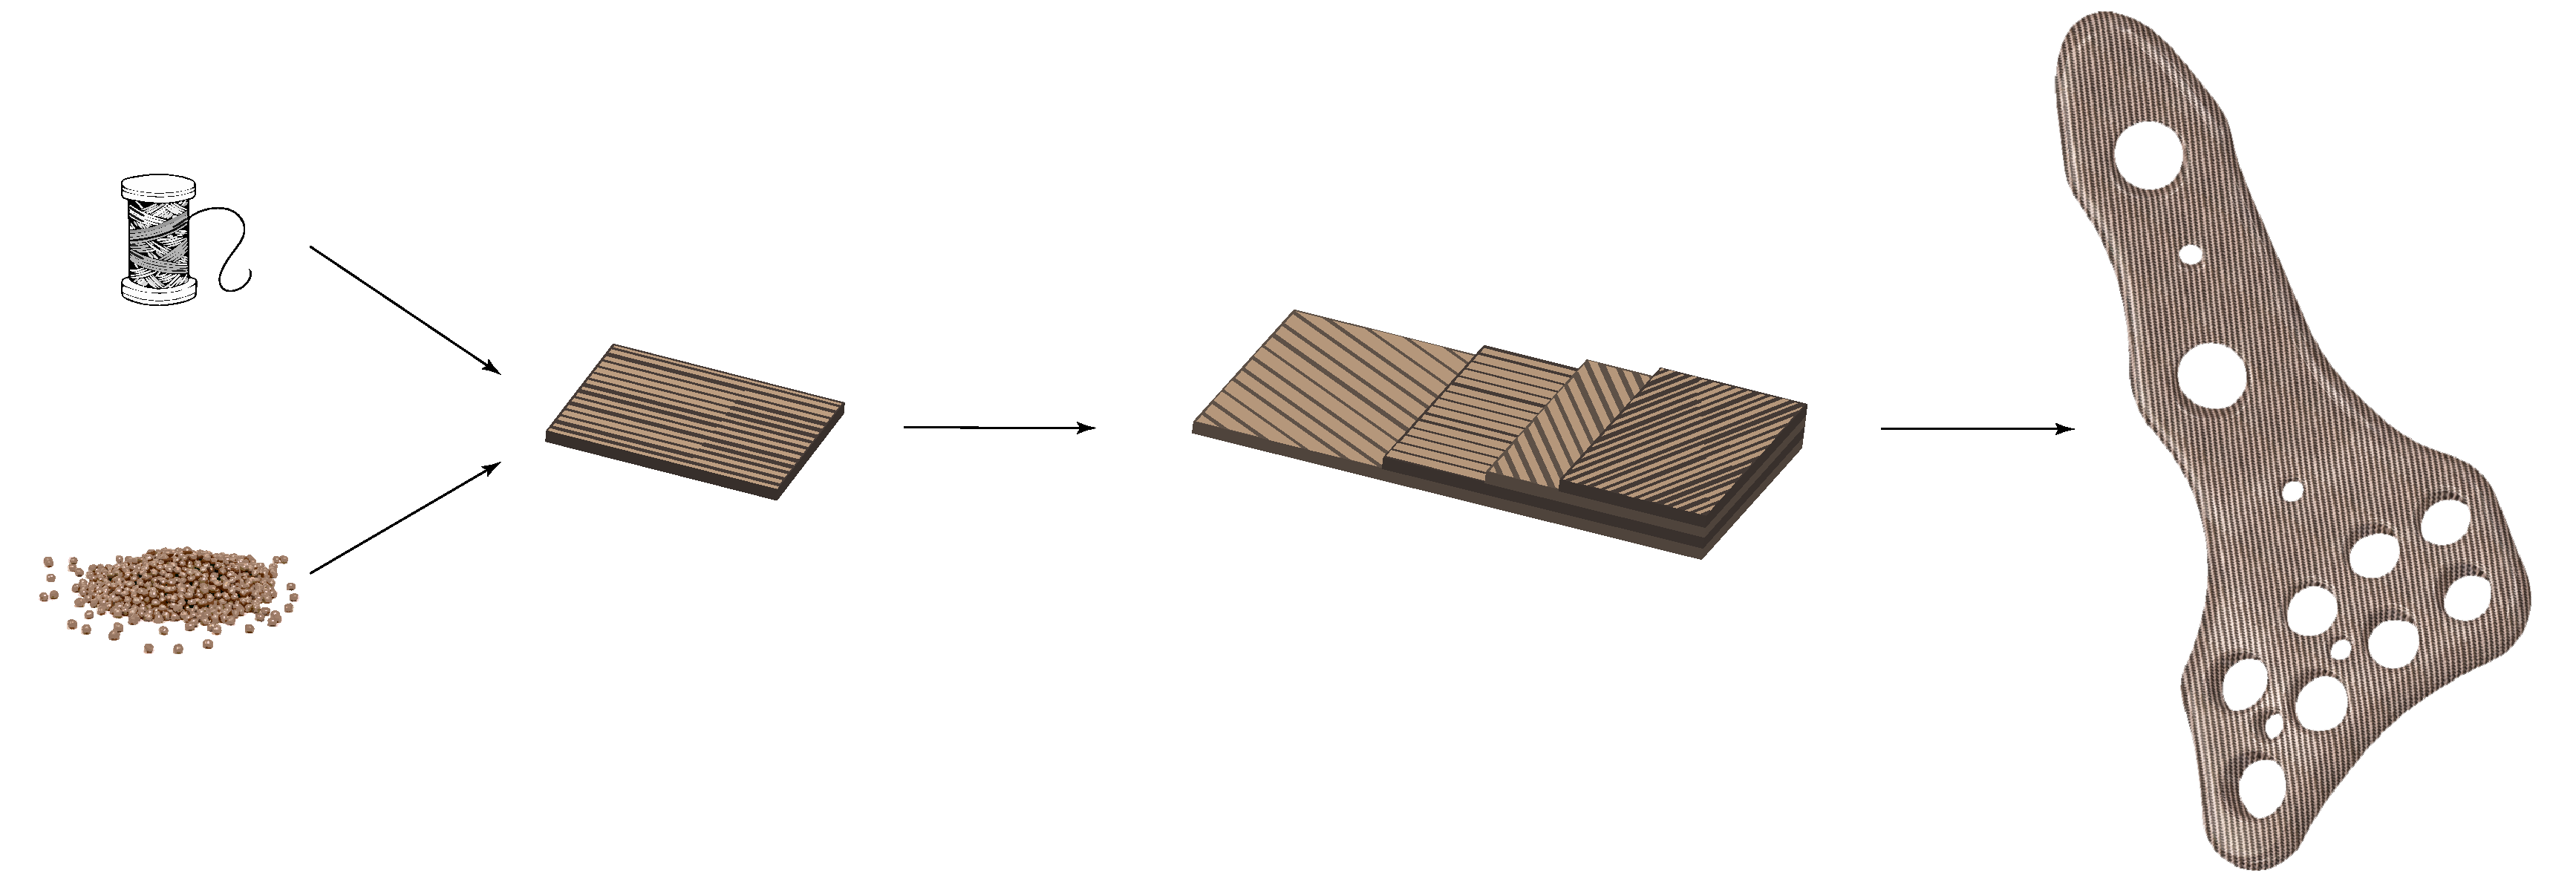
\includegraphics[width=\textwidth]{laminate_figures.pdf}
	\caption{Il comportamento meccanico della struttura finale alla macroscala è fortemente influenzato dai singoli componenti in cascata. Da sinistra: fibre continue di carbonio e pellet di polimero; singola lamina; piastra multi layer; placca ortopedica di fissaggio per il radio distale \citep{MUGNAI2018877}.}
\label{fig:laminates_general}
\end{figure*}

I compositi moderni si basano sull'utilizzo di una fase di rinforzo, tipicamente sotto forma di fibra, immersa in una matrice. Solitamente si utilizza una matrice polimerica e come fibre di rinforzo si possono usare vetro, carbonio, aramide ed altri. Esistono diversi metodi per disporre le fibre e la loro distribuzione influenza il comportamento globale. 

Mettendo insieme più strati di materiale composito si ottiene un pacchetto che prende il nome di composito laminato.

Il problema può essere diviso su tre scale di grandezza differenti: il comportamento della struttura finale (macroscala) dipende dal laminato che a sua volta è influenzato dalle singole lamine (mesoscala). A loro volta il comportamento è determinato dai singoli costituenti e dalla loro composizione (microscala). Una rappresentazione schematica è data in \cref{fig:laminates_general}.


\subsection{Regola delle miscele}

La singola lamina è composta da una matrice e dalle fibre di rinforzo con una frazione volumetrica precisa. Il primo passo è quello di omogenizzare le proprietà materiali del singolo strato. Consideriamo una fibratura tale da garantire una simmetria trasversalmente isotropa e con direzione di isotropia l'asse della fibra. 

Per arrivare alle proprietà omogenizzate del singolo layer è possibile applicare la regola delle miscele \citep{Kollar:1}.

Considerando un volume globale del composito dato dalla somma del volume della matrice e di quello del rinforzo e assumendo un'adesione corretta tra i due è possibile calcolare analiticamente i moduli risultanti. Valgono le frazioni volumetriche:

\begin{equation}
v_m+f_f=1   
\end{equation}

Ed è possibile esprime le proprietà materiali risultanti in funzione della frazione volumetrica di fibre ($f_f$) e delle proprietà materiali dei singoli costituenti, come espresso nelle \cref{eq:E1,eq:E2,eq:G12,eq:nu12,eq:nu23,}. 

\begin{equation}
E_1=f_f E_f+\left(1-f_f\right)E_m
\label{eq:E1}
\end{equation}

\begin{equation}
{E_2}=E_3=\left({1-f_f\over E_m}+{f_f\over E_f}\right)^{-1}
\label{eq:E2}
\end{equation}

\begin{equation}
G_{12}=\left(\frac{v_{m}}{G_{m}}+\frac{v_{f}}{G_{f}}\right)^{-1}
\label{eq:G12}
\end{equation}

\begin{equation}
\nu_{12}=v_{f} \nu_{f}+v_{m} \nu_{m}
	\label{eq:nu12}
\end{equation}

\begin{equation}
\nu_{23}=\frac{E_{2}}{2 G_{23}}-1=\frac{E_{2}}{2 G_{12}}-1
	\label{eq:nu23}
\end{equation}

È possibile considerare una matrice di cedevolezza del tipo in \cref{eq:SS}

\begin{equation}
\begin{bmatrix}
	\frac{1}{E_{1}} & -\frac{\nu_{21}}{E_{2}} & -\frac{\nu_{31}}{E_{3}} & 0 & 0 & 0 \\
	-\frac{\nu_{12}}{E_{1}} & \frac{1}{E_{2}} & -\frac{\nu_{32}}{E_{3}} & 0 & 0 & 0 \\
	-\frac{\nu_{13}}{E_{1}} & -\frac{\nu_{23}}{E_{2}} & \frac{1}{E_{3}} & 0 & 0 & 0 \\
	0 & 0 & 0 & \frac{1}{G_{23}} & 0 & 0 \\
	0 & 0 & 0 & 0 & \frac{1}{G_{13}} & 0 \\
	0 & 0 & 0 & 0 & 0 & \frac{1}{G_{12}}
\end{bmatrix}
\label{eq:SS}
\end{equation}

\subsection{Teoria dei laminati sottili ??}

\textcolor{blue}{\lipsum[1-2]}




\section{Proprietà dei costituenti}

\begin{table}[bt!]
	\centering
	\captionsetup{justification=centering}
	
	\caption{Parametri materiali \citep{Gallagher}}

	\begin{tabular}{l l l}
		\toprule
		CF & PEEK\\
		\midrule
		$E_{f}=236$ GPa & $E_{m}=$ 4 GPa   \\
		$\nu_{f}= 0.2$ & $\nu_{m}= 0.36$ \\
		$G_f=27.6 $ GPa & $G_m=1.47$ GPa \\
		\bottomrule
	\end{tabular}
	\label{tab:parametri}
\end{table}

Introduci REGOLA DELLE MISCELE

Fissata una fiber fraction di $ff=0.62$.  

PLOTTA E1 ed E2 rispetto alla variazione del fiber fraction ??

TEST SU LAMINATI CON DIFFERNTI PROPRIETà ??  EVENTUALMENTE USA IL CASO SPECIALE DELLE TENSIONI NELLO SPESSORE

\textcolor{blue}{\lipsum[1-2]}

\begin{table}[bt!]
	\centering
	\captionsetup{justification=centering}
	
	\caption{Risultati applicando la regola delle miscele}
	
	\begin{tabular}{l l l}
		\toprule
				$ff$  & 0.62 \\
						\toprule
		$E_{1}$  & 147.96 GPa  \\
		$E_{2}$  & 10.83 GPa  \\
		$\nu_{12}$ & $0.26$ \\
		$G_{12}$ & 4.24 GPa \\
		\bottomrule
	\end{tabular}
	\label{tab:miscele}
\end{table}

\section{Layout del laminato}

\begin{figure*}[bt!]
	\centering
	\begin{subfigure}[t]{0.24\textwidth}
		\centering
		
		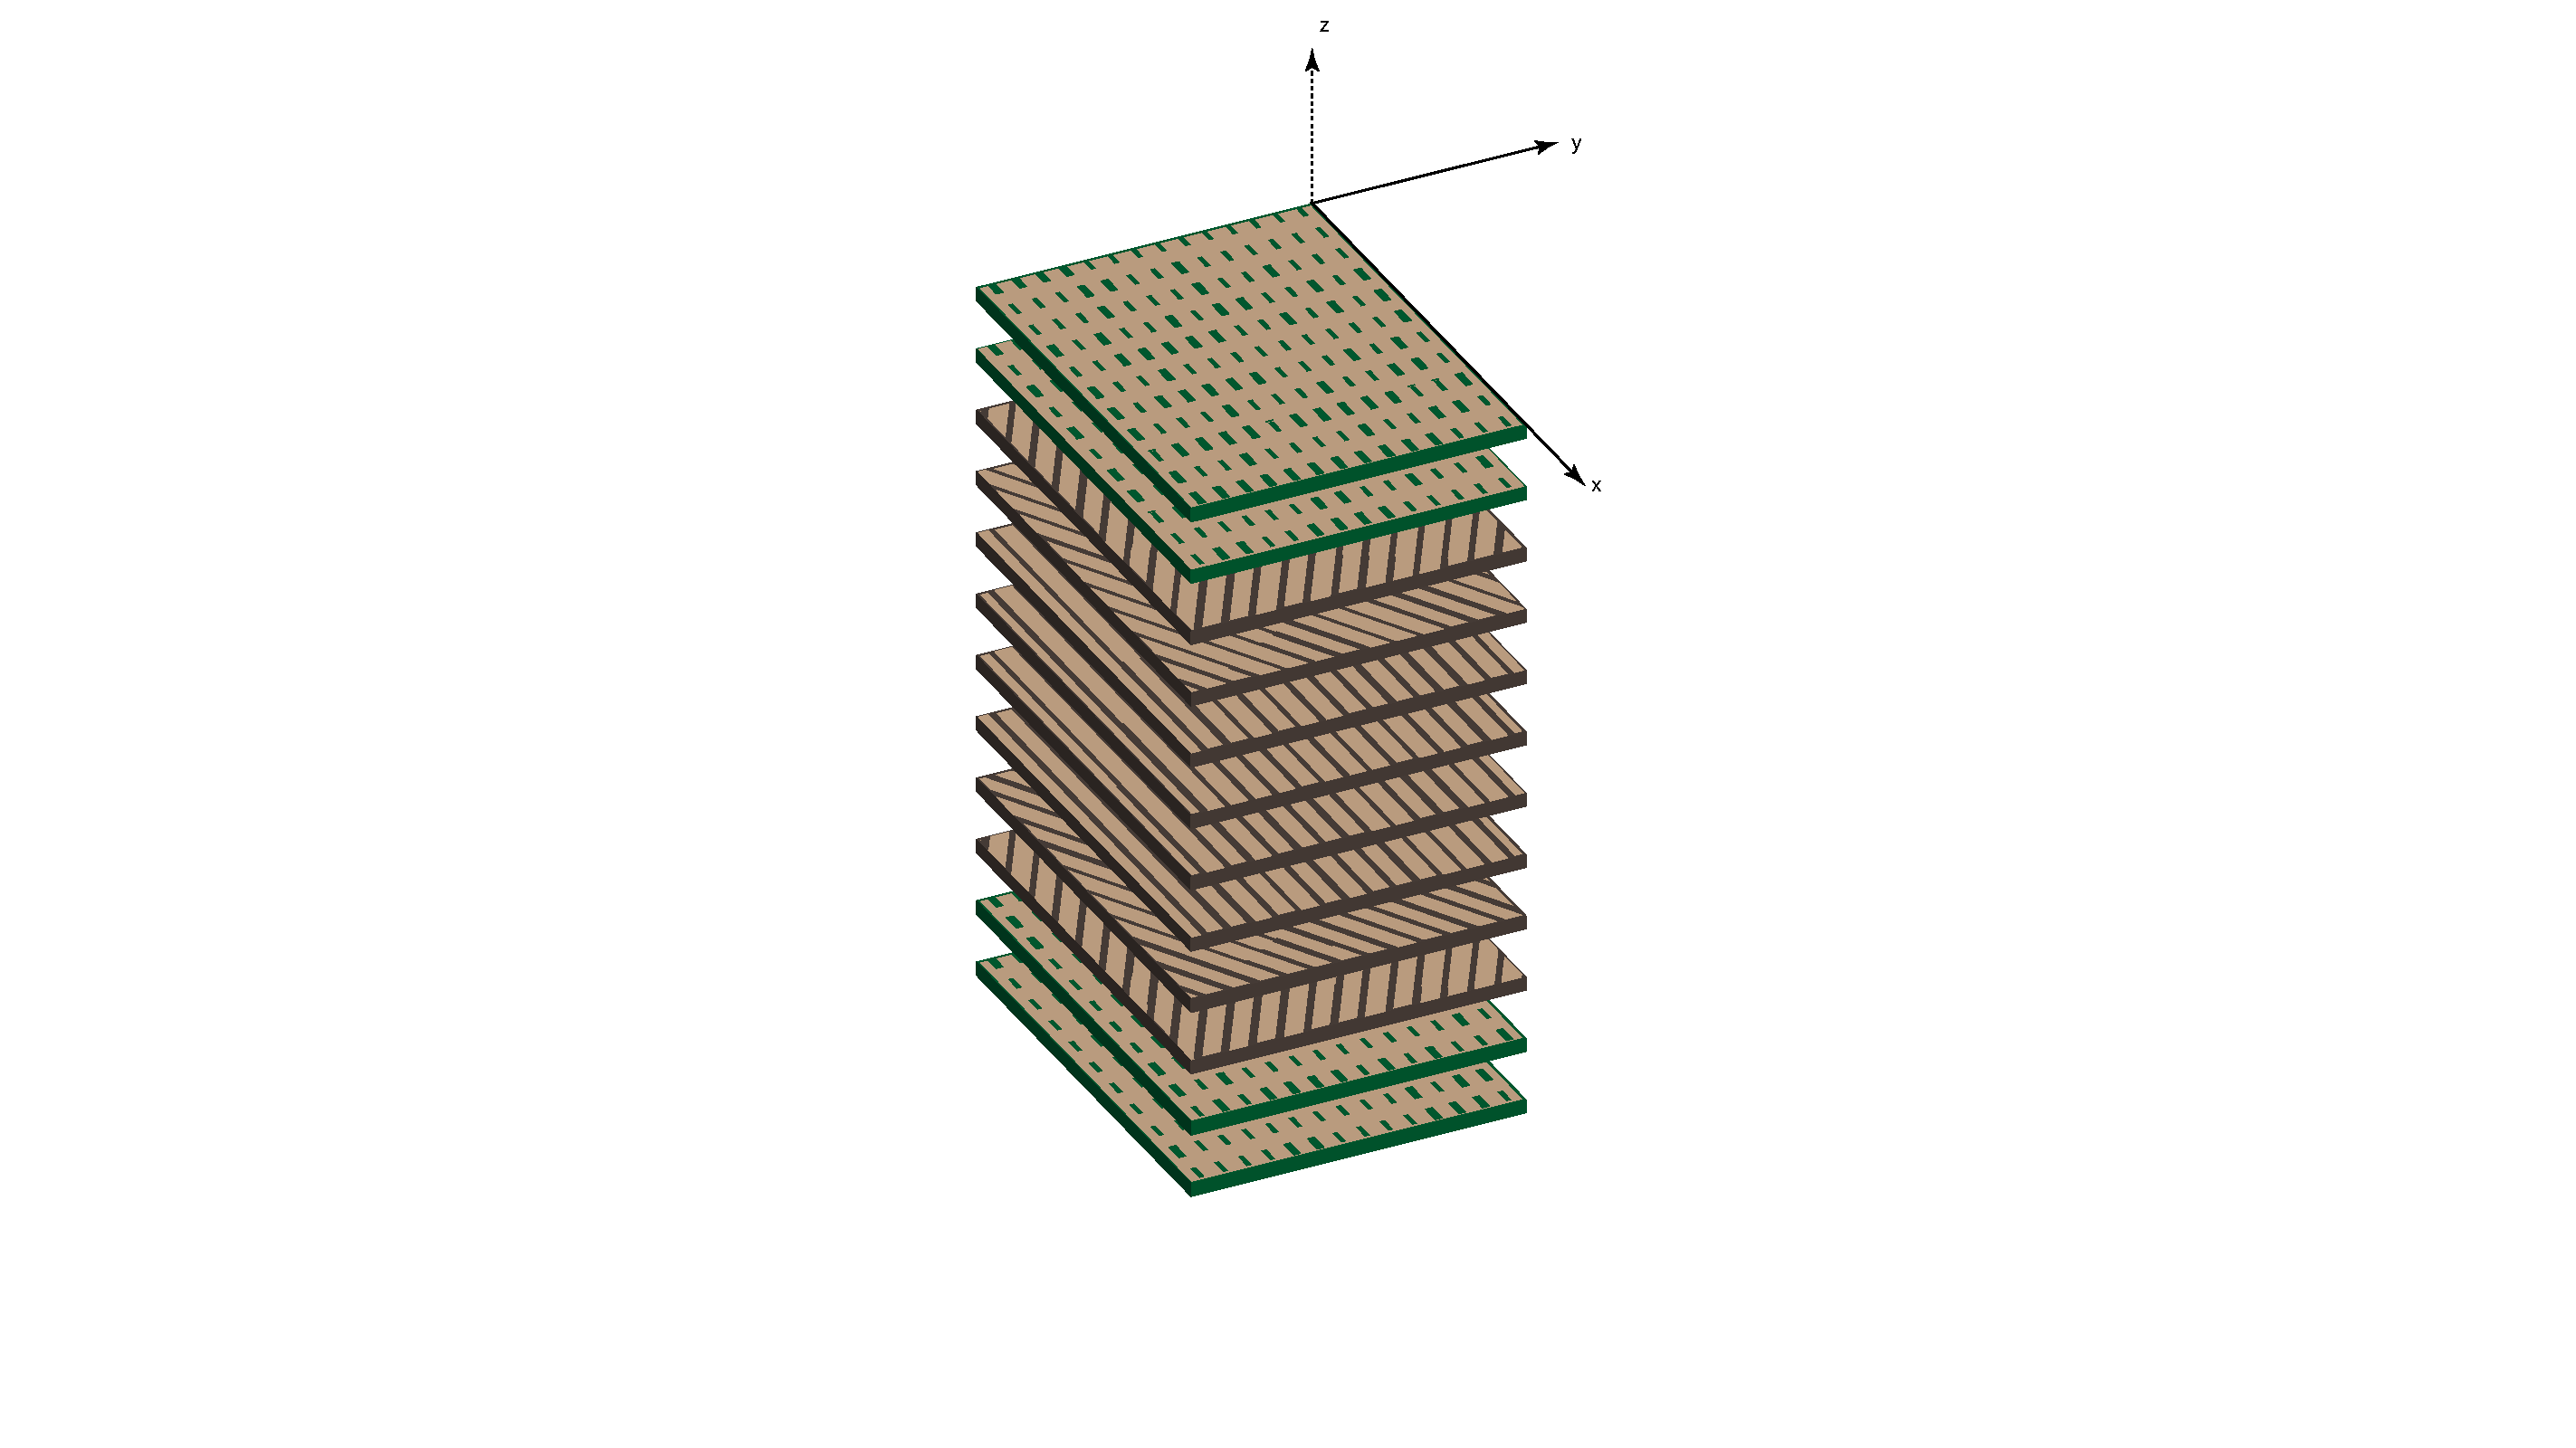
\includegraphics[width=\textwidth]{struct1.pdf}
		\caption{$[\alpha /-\alpha / 30 /-30 / 0_{2}]_{\mathrm{s}}$ }
		
	\end{subfigure}
	\hfill
	\begin{subfigure}[t]{0.24\textwidth}
		\centering
		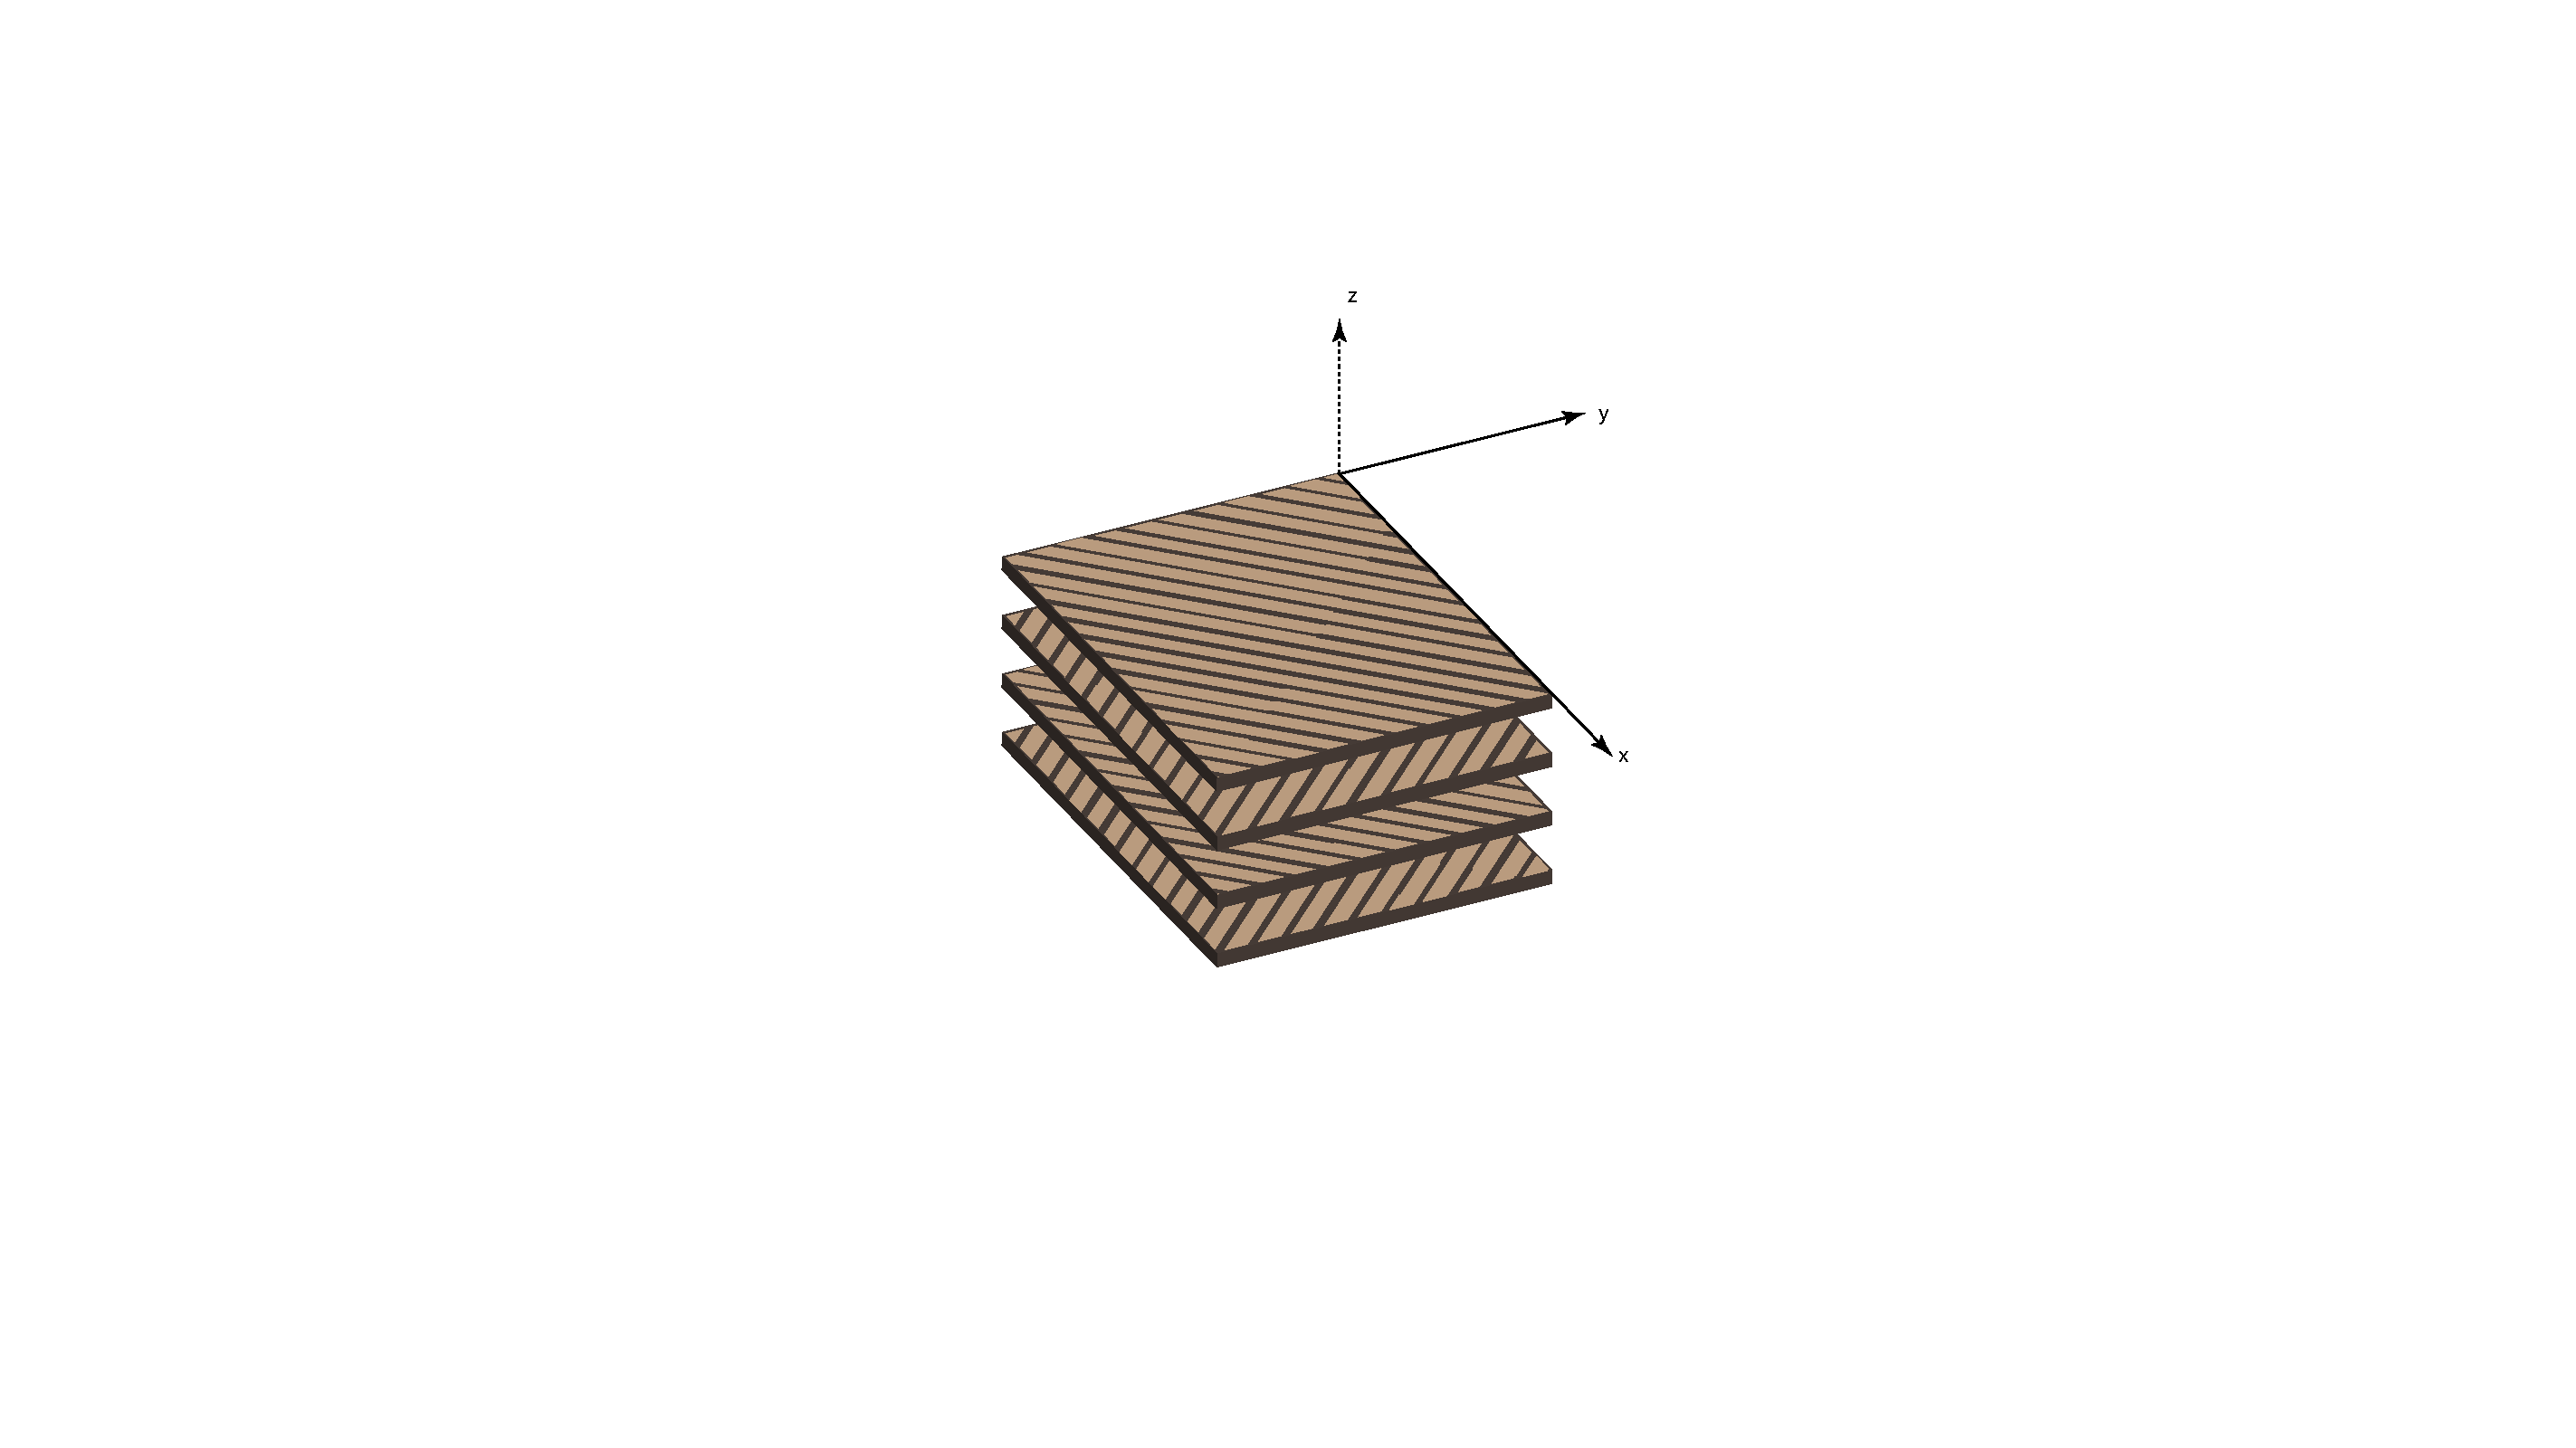
\includegraphics[width=\textwidth]{struct2.pdf}
		\caption{$[-45 / 45 /-45 / 45]$}
		
	\end{subfigure}
	\hfill
	\begin{subfigure}[t]{0.24\textwidth}
		\centering
		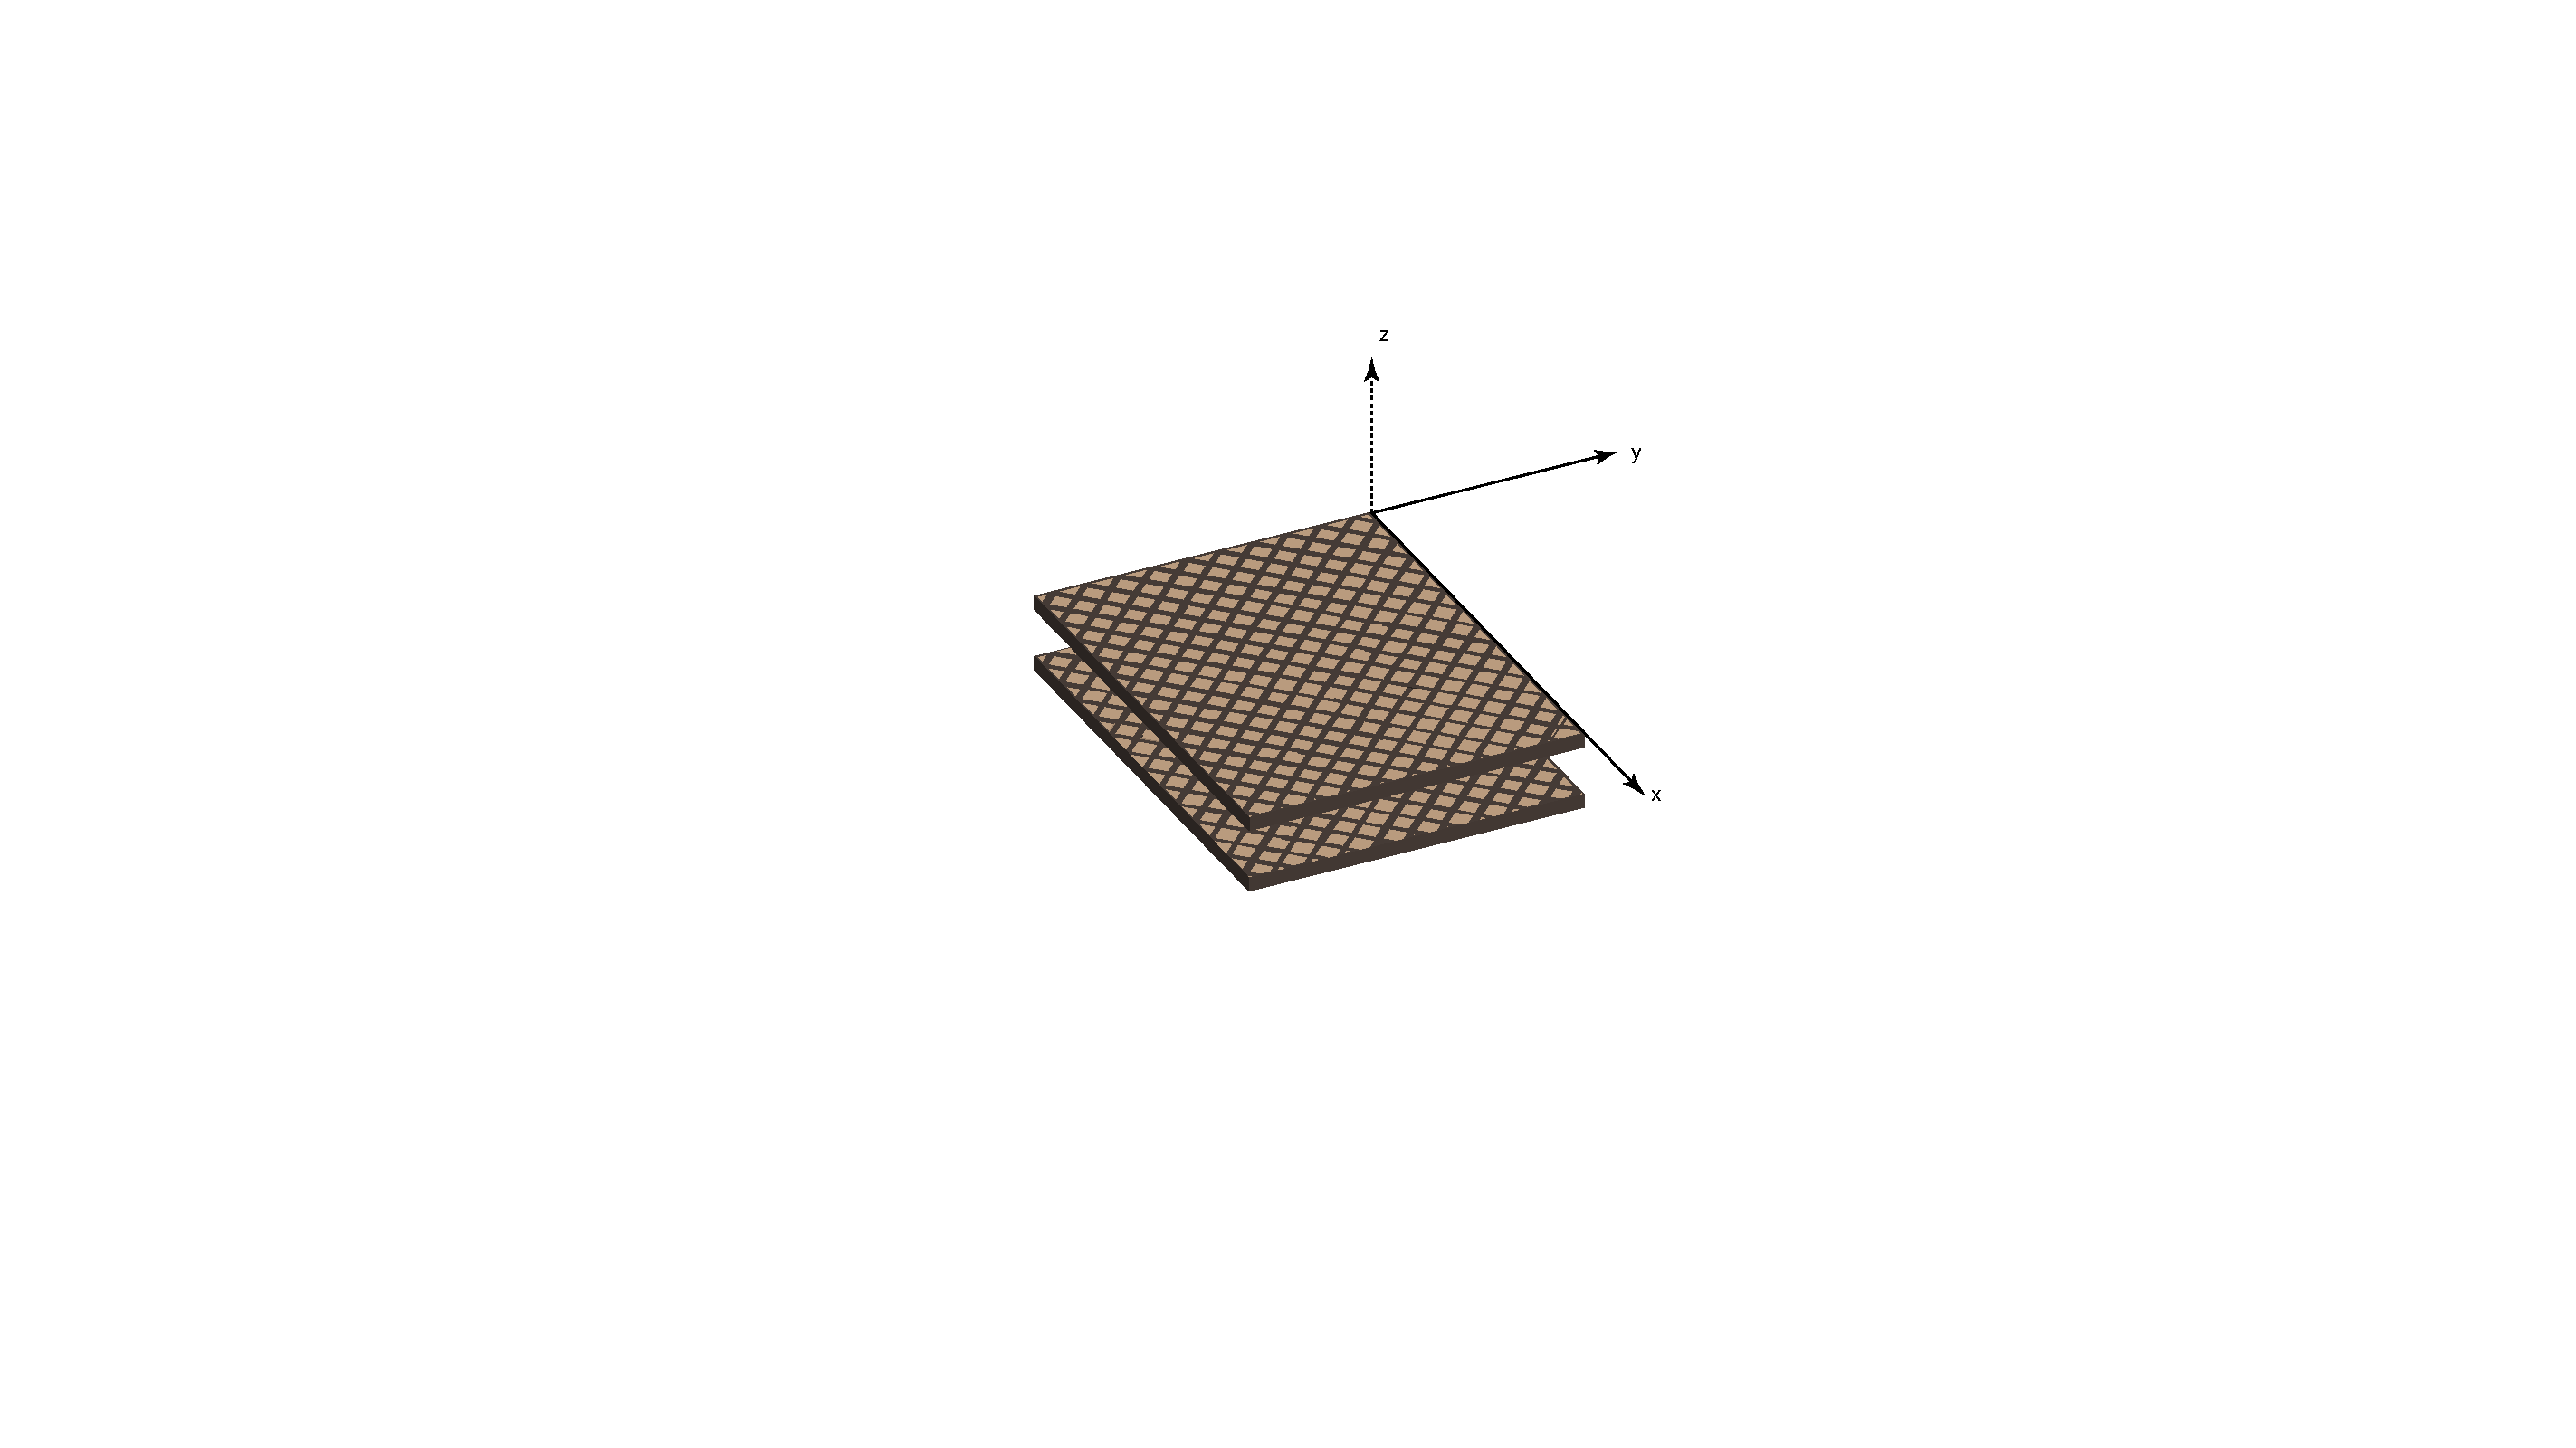
\includegraphics[width=\textwidth]{struct3.pdf}
		\caption{$[\pm 45^{f} / \pm 45^{f}]$}
		
	\end{subfigure}
	\hfill
	\begin{subfigure}[t]{0.24\textwidth}
		\centering
		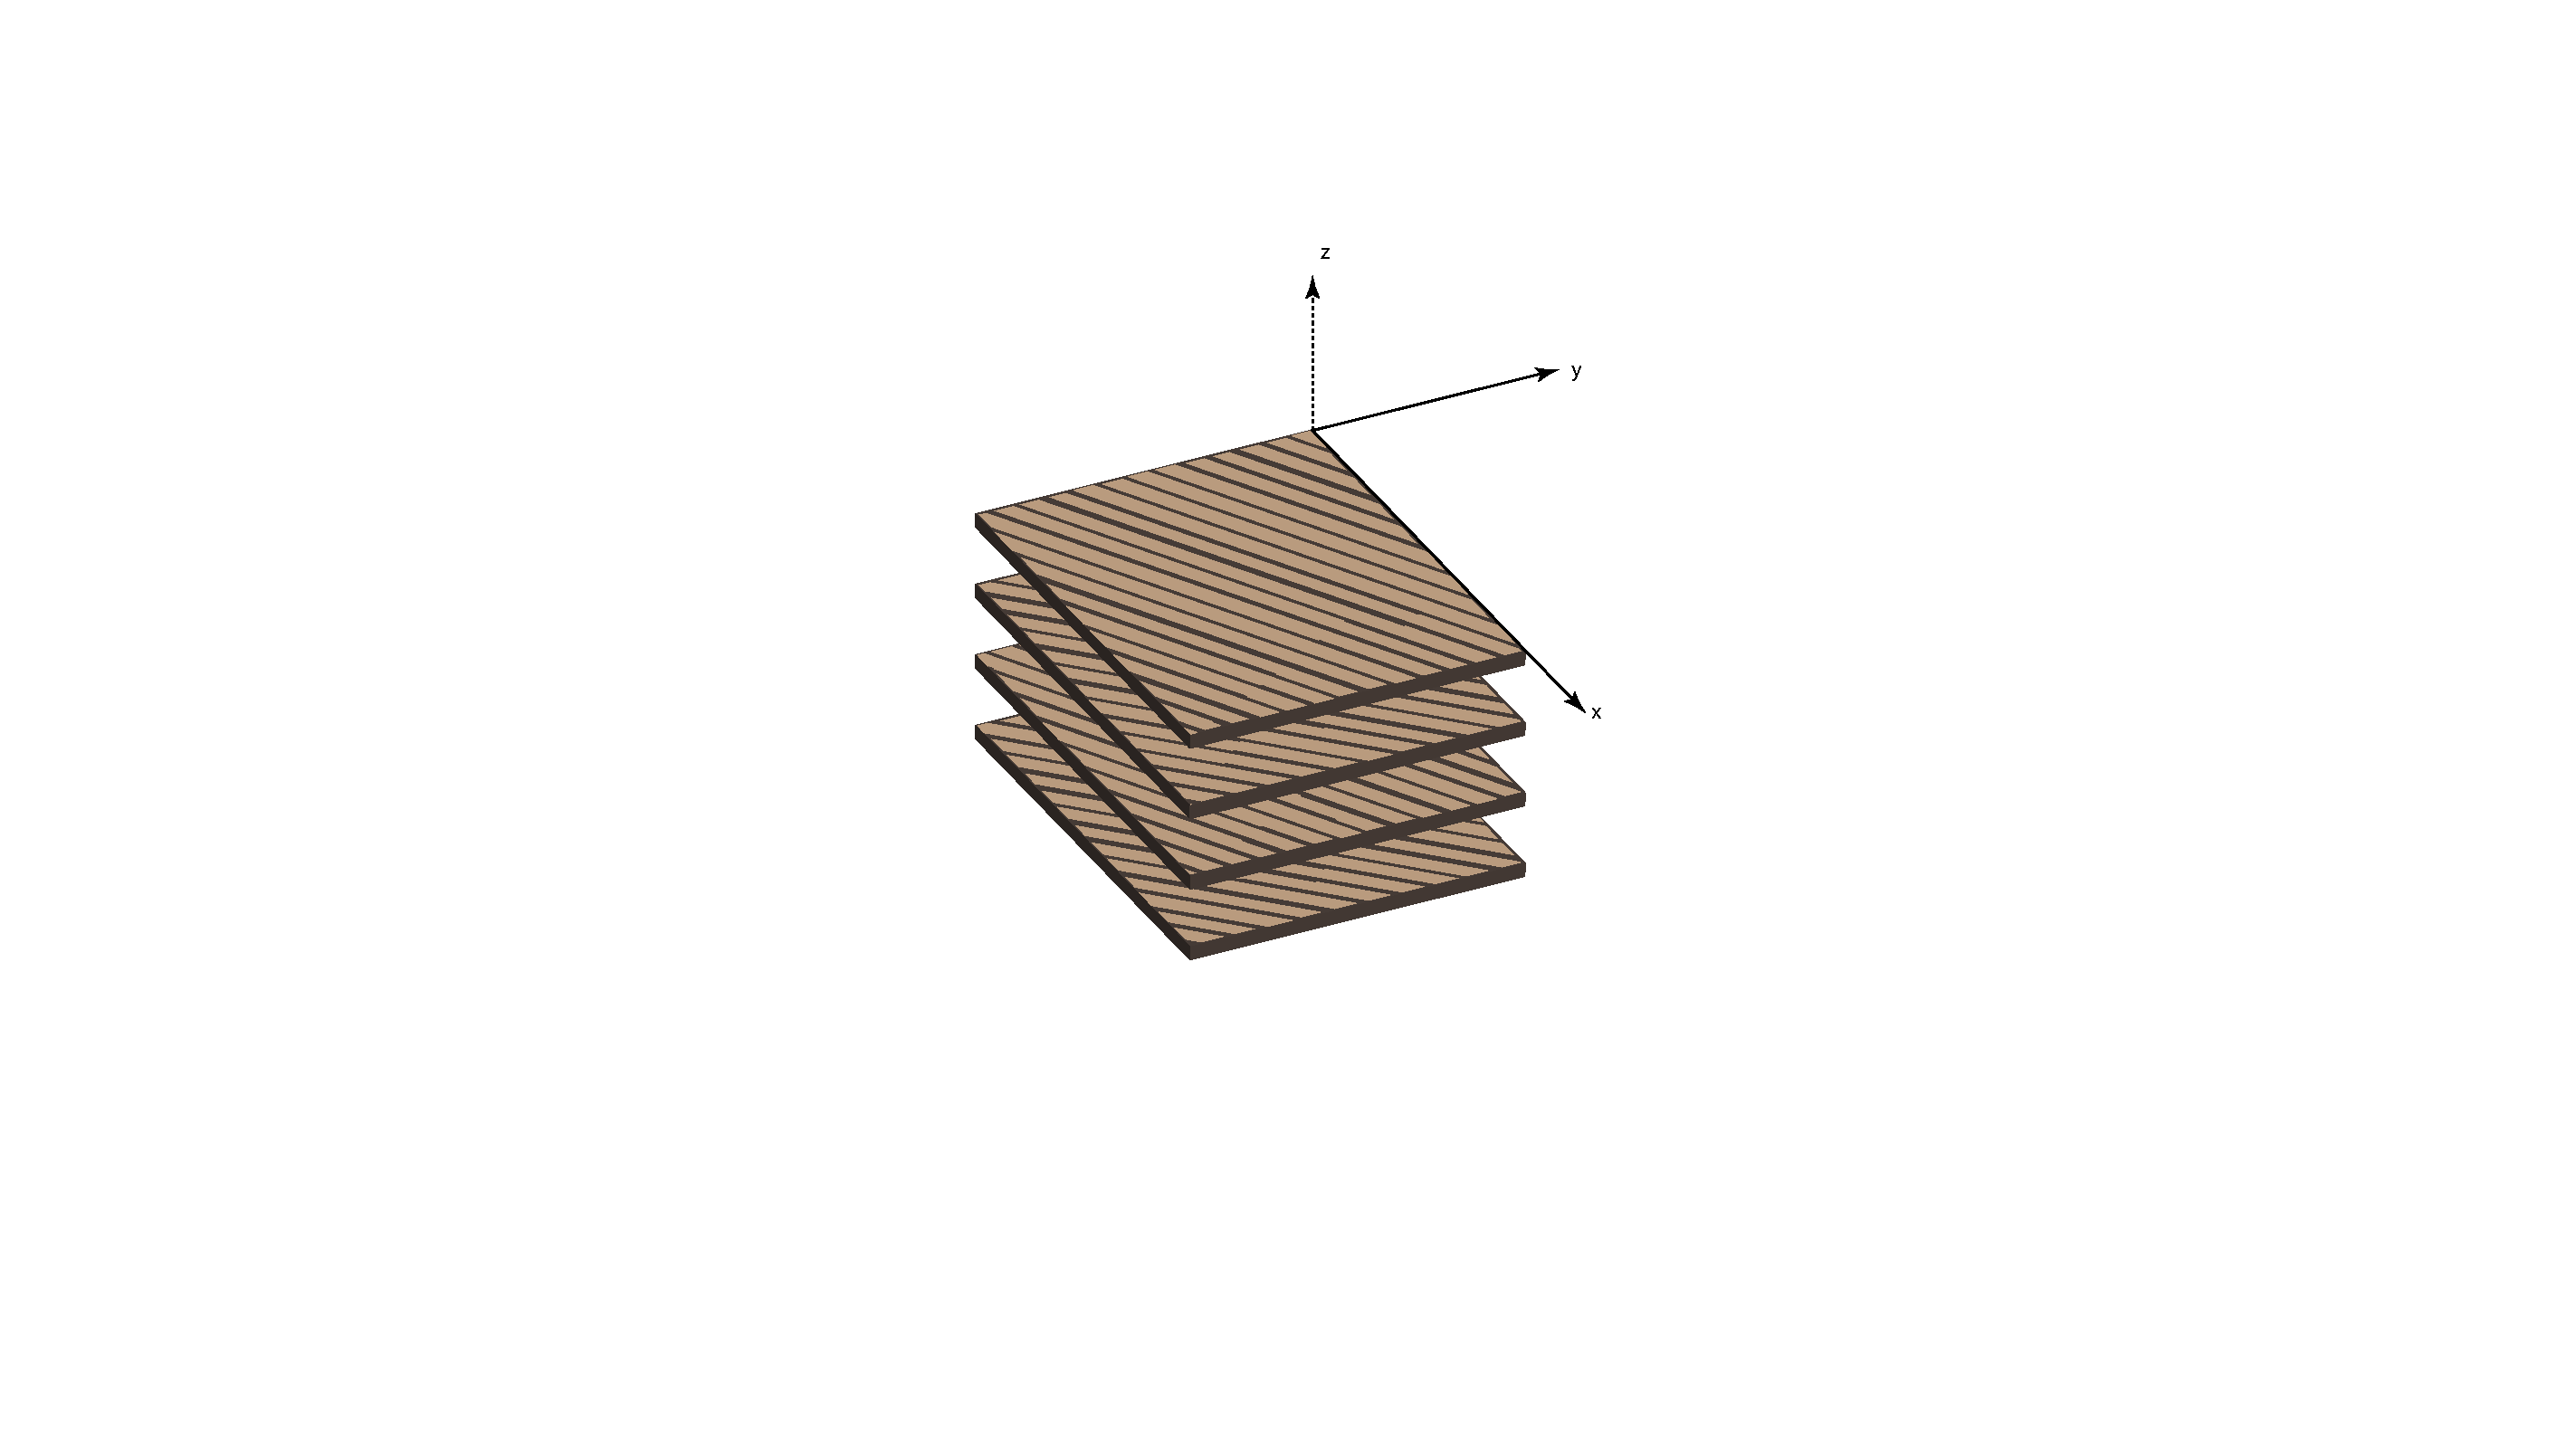
\includegraphics[width=\textwidth]{struct4.pdf}
		\caption{$[-30 /-45 /-30 /-45]$}
		
	\end{subfigure}
	\hfill
	\caption{Differenti layout di laminato }
	\label{fig:laminates}
\end{figure*}

Vengono affrontati 4 casi:

\begin{enumerate}[label=(\alph*)]
	\item $[\alpha /-\alpha / 30 /-30 / 0_{2}]_{\mathrm{s}}$ con $\alpha\in\left[0^\circ;90^\circ\right]$
	\item $[-45 / 45 /-45 / 45]$
	\item $[\pm 45^{f} / \pm 45^{f}]$
	\item $[-30 /-45 /-30 /-45]$
\end{enumerate}

Un'illustrazione rappresentativa dei differenti layout è presente in \cref{fig:laminates}.

Vengono affrontati anche due elementi strutturali differenti:
\begin{itemize}
\item Elemento tipo piastra
\item Elemento tipo cilindro
\end{itemize}

\begin{figure*}[bt!]
	\centering
	\begin{subfigure}[t]{0.24\textwidth}
		\centering

 \includegraphics[width=\textwidth]{plate_.pdf}
 				\caption{Elemento tipo piastra}
		\label{fig:y equals x}
	\end{subfigure}
	\hfill
	\begin{subfigure}[t]{0.24\textwidth}
		\centering
		\includegraphics[width=\textwidth]{/first_test/alpha=40.pdf}
		\caption{Elemento tipo piastra deformato (caso \cref{sec:plate_A}  con $\alpha=40^\circ$ )}
		\label{fig:five over x}
	\end{subfigure}
	\hfill
	\begin{subfigure}[t]{0.24\textwidth}
		\centering
 \includegraphics[width=\textwidth]{cyl_.pdf}
\caption{Elemento tipo cilindro}
		\label{fig:three sin x}
	\end{subfigure}
	\hfill
	\begin{subfigure}[t]{0.24\textwidth}
	\centering
 \includegraphics[width=\textwidth]{/more_test/cyl_30_45_30_45.pdf}
	\caption{Elemento tipo cilindro deformato (caso \cref{sec:cyl_D}}
	\label{fig:five ove x}
\end{subfigure}
	\hfill
	\caption{Elementi strutturali}
	\label{fig:three graphs}
\end{figure*}



COMPLETA CON ELENCO PUNTATO E DIFFERENTI CASI 

PRESENTA I DUE DIFFERENTI ELEEMTNI STRUTTURALI
\textcolor{blue}{\lipsum[1-2]}





\subsection{Elemento tipo piastra}
\subsubsection{Caso (a)}
\label{sec:plate_A}

\begin{figure*}[bt!]
	\centering

	\begin{subfigure}[t]{0.3\textwidth}
		\centering
		\includegraphics[width=\textwidth]{/first_test/bothload/V_X.pdf}
		\caption{Spostamento lungo $\hat y$ del bordo con $y=0$ della piastra}
		
	\end{subfigure}
	\hfill
	\begin{subfigure}[t]{0.3\textwidth}
		\centering
\includegraphics[width=\textwidth]{/first_test/bothload/W_Y.pdf}
		
		\caption{Effetto torsionale, spostamento lungo $\hat z$ del bordo estremale della piastra ($x=L$)}
		
	\end{subfigure}
	\hfill
	\begin{subfigure}[t]{0.3\textwidth}
		\centering
		\includegraphics[width=\textwidth]{/first_test/bothload/W_X.pdf}
		\caption{Effetto flessionale, spostamento lungo $z$ del bordo $y=0$ della piastra}
		
	\end{subfigure}
	\hfill
	\caption{Risultati caso (a) per un elemento strutturale tipo piastra con entrambi i carichi (\cref{sec:plate_A})}
	\label{fig:plate_A_both_load}
\end{figure*}


\begin{figure*}[bt!]
	\centering
	
	\begin{subfigure}[t]{0.3\textwidth}
		\centering
		\includegraphics[width=\textwidth]{/first_test/transversal_load/V_X.pdf}
		\caption{Spostamento lungo $\hat y$ del bordo con $y=0$ della piastra}
		
	\end{subfigure}
	\hfill
	\begin{subfigure}[t]{0.3\textwidth}
		\centering
		\includegraphics[width=\textwidth]{/first_test/transversal_load/W_Y.pdf}
		
		\caption{Effetto torsionale, spostamento lungo $\hat z$ del bordo estremale della piastra ($x=L$)}
		
	\end{subfigure}
	\hfill
	\begin{subfigure}[t]{0.3\textwidth}
		\centering
		\includegraphics[width=\textwidth]{/first_test/transversal_load/W_X.pdf}
		\caption{Effetto flessionale, spostamento lungo $z$ del bordo $y=0$ della piastra}
		
	\end{subfigure}
	\hfill
	\caption{Risultati caso (a) per un elemento strutturale tipo piastra con carichi tipo trasversale (\cref{sec:plate_A})}
	\label{fig:plate_A_transload_load}
\end{figure*}

\begin{figure*}[bt!]
	\centering
	
	\begin{subfigure}[t]{0.3\textwidth}
		\centering
		\includegraphics[width=\textwidth]{/first_test/axial_load/V_X.pdf}
		\caption{Spostamento lungo $\hat y$ del bordo con $y=0$ della piastra}
		
	\end{subfigure}
	\hfill
	\begin{subfigure}[t]{0.3\textwidth}
		\centering
		\includegraphics[width=\textwidth]{/first_test/axial_load/W_Y.pdf}
		
		\caption{Effetto torsionale, spostamento lungo $\hat z$ del bordo estremale della piastra ($x=L$)}
		
	\end{subfigure}
	\hfill
	\begin{subfigure}[t]{0.3\textwidth}
		\centering
		\includegraphics[width=\textwidth]{/first_test/axial_load/W_X.pdf}
		\caption{Effetto flessionale, spostamento lungo $z$ del bordo $y=0$ della piastra}
		
	\end{subfigure}
	\hfill
	\caption{Risultati caso (a) per un elemento strutturale tipo piastra con carichi tipo assiale(\cref{sec:plate_A})}
	\label{fig:plate_A_axial_load}
\end{figure*}


\textcolor{blue}{\lipsum[1-2]}


\subsubsection{Caso (b)}
\textcolor{blue}{\lipsum[1-2]}
\subsubsection{Caso (c)}
\textcolor{blue}{\lipsum[1-2]}
\subsubsection{Caso (d)}
\textcolor{blue}{\lipsum[1-2]}

\subsection{Elemento tipo cilindro}

\subsubsection{Caso (a)}
\textcolor{blue}{\lipsum[1-2]}
\subsubsection{Caso (b)}
\label{sec:cyl_B}
\textcolor{blue}{\lipsum[1-2]}
\subsubsection{Caso (c)}
\label{sec:cyl_C}
\textcolor{blue}{\lipsum[1-2]}
\subsubsection{Caso (d)}
\label{sec:cyl_D}
\textcolor{blue}{\lipsum[1-2]}


\section{Spessore della piastra}

Consideriamo un ulteriore caso con un layout $[10 /-10 / 30 /-30 / 0_2]_{\mathrm{s}}$ illustrato in \cref{fig:last_case_schema}. 

\begin{figure*}[bt!]
	\centering
	\begin{subfigure}[t]{0.3\textwidth}
		\centering
		
		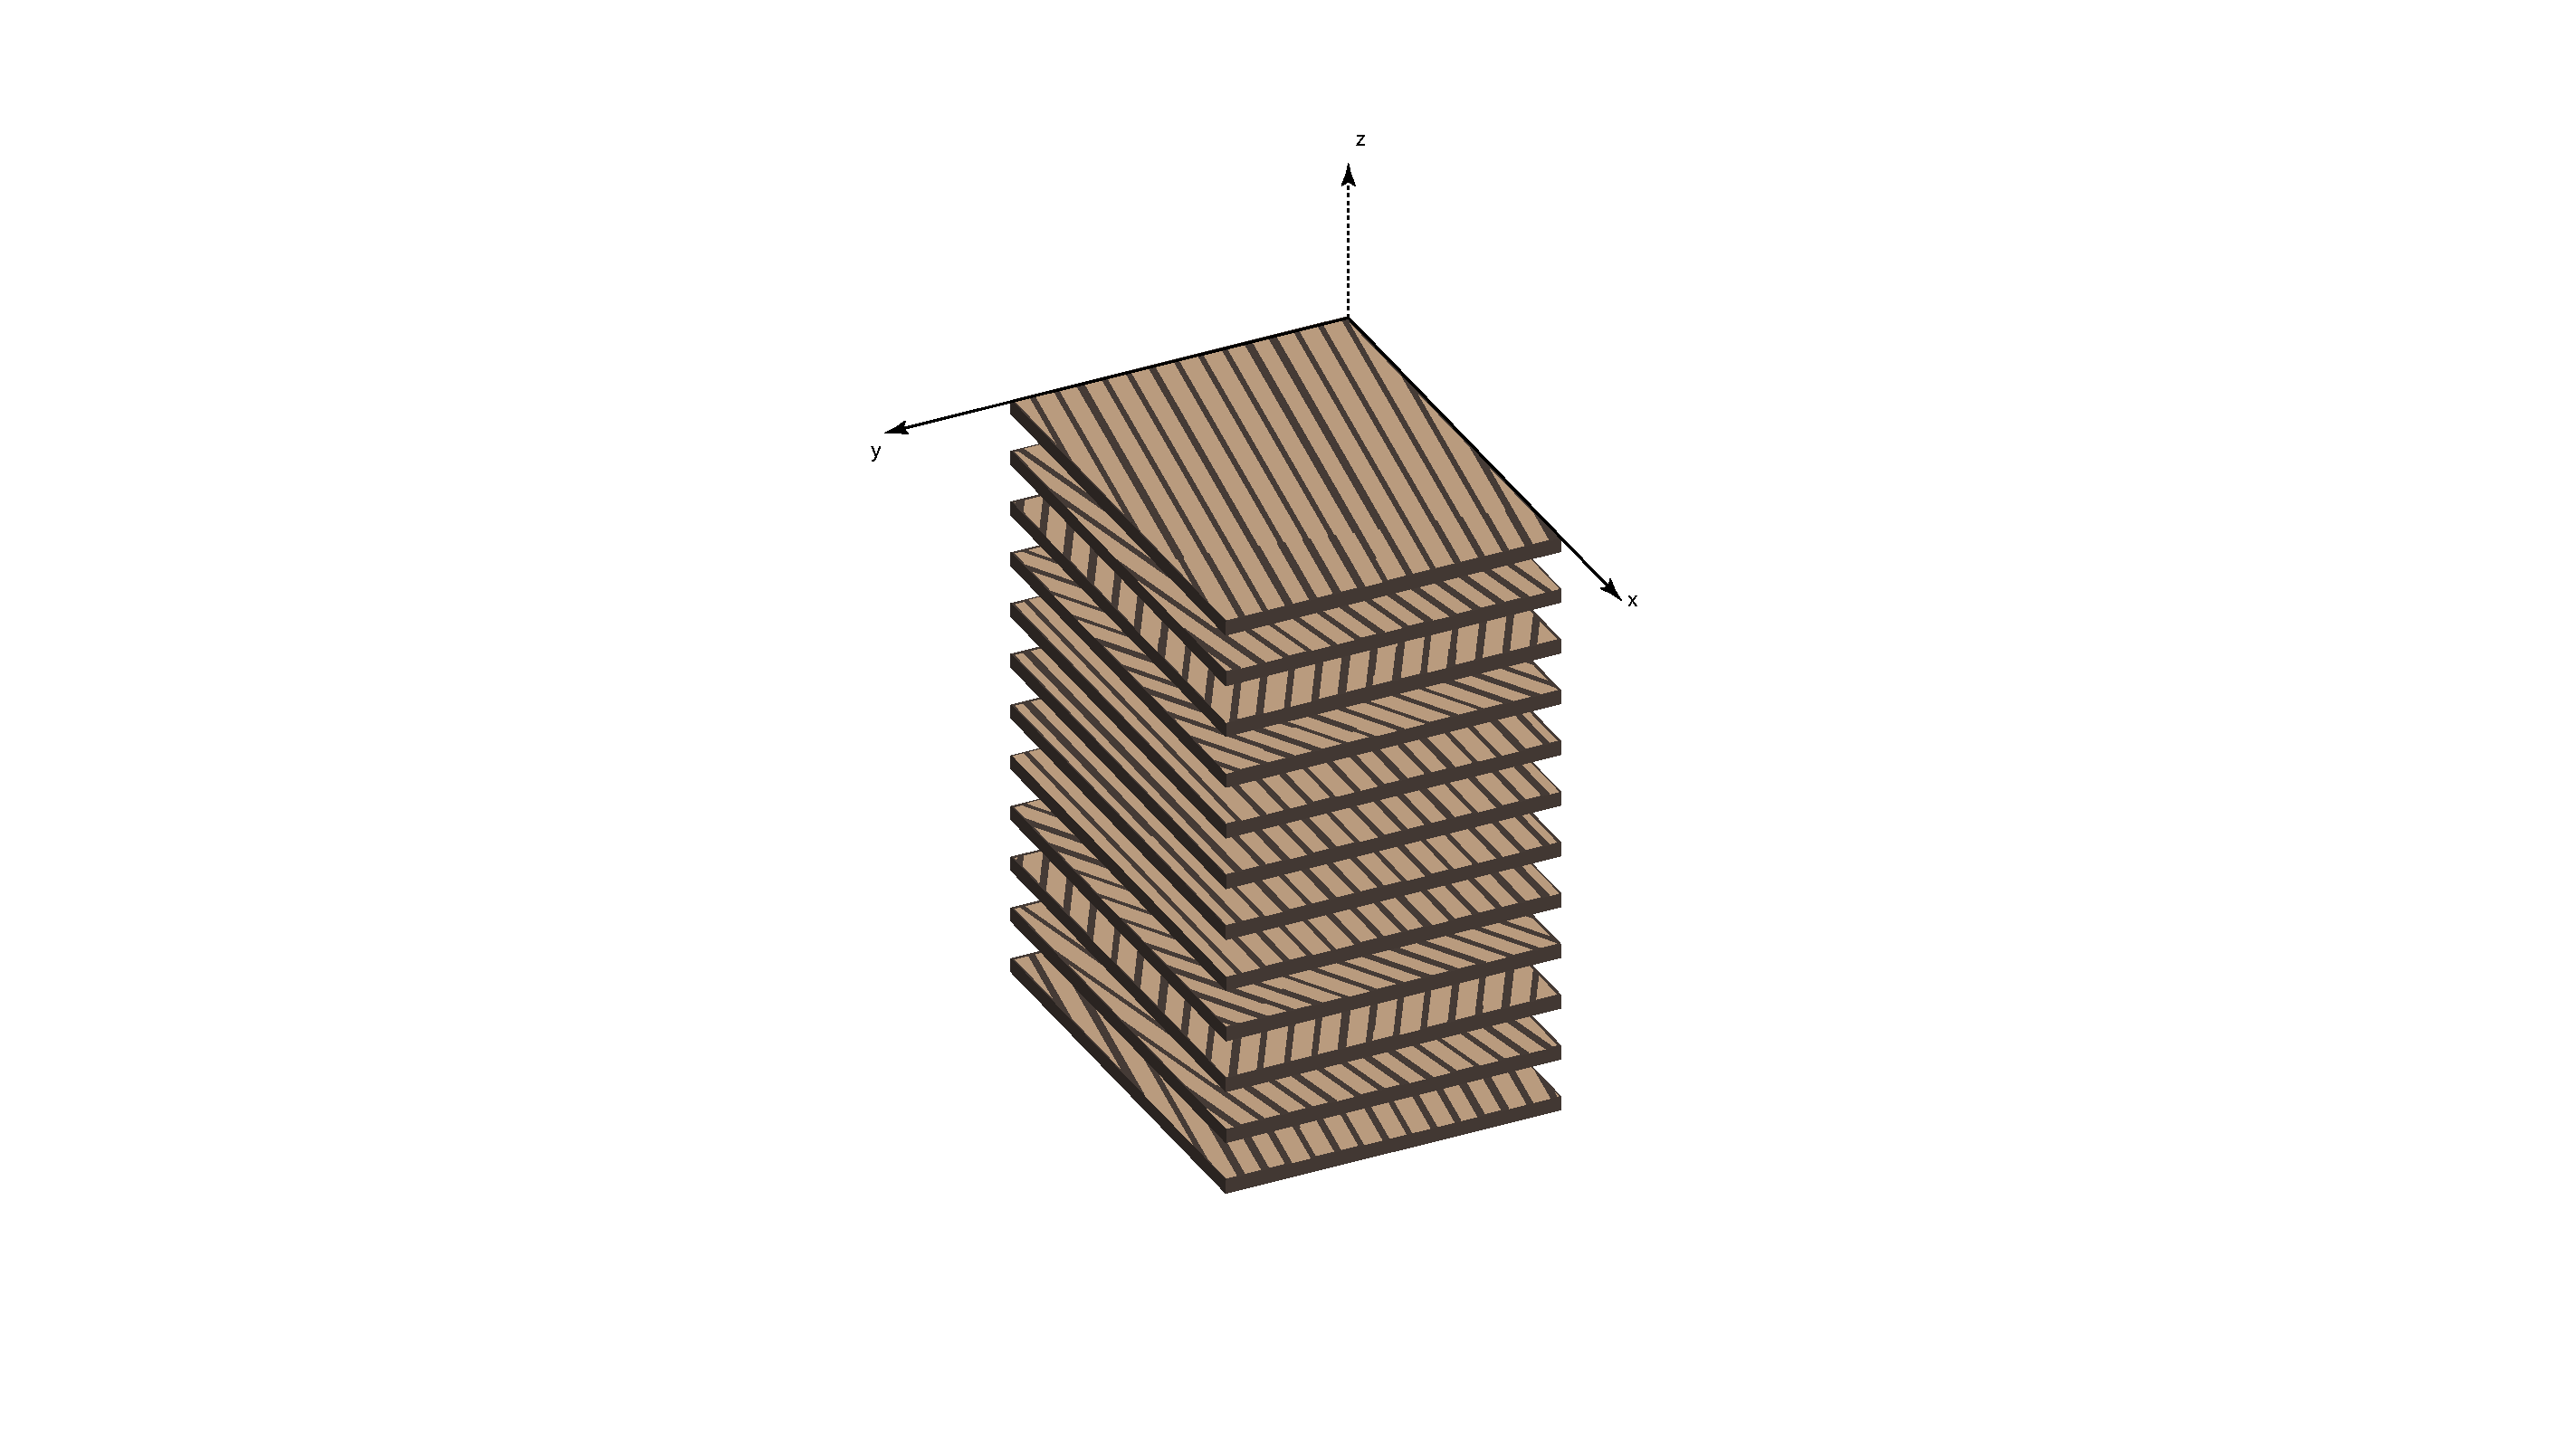
\includegraphics[width=\textwidth]{struct5.pdf}
		\caption{Descrizione}
			\label{fig:last_case_schema}
	\end{subfigure}
	\hfill
	\begin{subfigure}[t]{0.3\textwidth}
		\centering
		METTI FIGURA DI PROFILO CON RETTANGOLI CON GRADI
		%\includegraphics[width=\textwidth]{V_X=.pdf}
		\caption{Descrizione}
		
	\end{subfigure}
	\hfill
	\begin{subfigure}[t]{0.3\textwidth}
		\centering
		%\includegraphics[width=\textwidth]{W_Y=.pdf}
		\caption{Descrizione}
		
	\end{subfigure}
	\hfill
	\caption{ DESCRIZIONE }
	\label{fig:last_case}
\end{figure*}

\textcolor{blue}{\lipsum[1-2]}


\section{Conclusioni}


CMPOMPLETA

Conoscere la risposta di elementi strutturali può essere utile per modellare correttamente una determinata struttura protesica e per fare studi dettagliati  di danno.

textcolor{blue}{\lipsum[1-2]}
\section{Metodi}

\textcolor{blue}{\lipsum[1-2]}


\section{Disponibilità del codice e materiale aggiuntivo}

Tutto il codice, le immagini, file di processamento e risultati ottenuti sono disponibili alla repository online al link: \url{https://github.com/mastroalex/comp-lam}. 

Il codice 


\subsection{Lista delle abbreviazioni}

\begin{itemize}
	\item CF, carbon fiber
\end{itemize}
 


%% Specify your .bib file name here, without the extension
%\newpage
%\onecolumn

\newpage
\bibliography{paper-refs}




\end{document}
